%! TEX root = ../dsa-mini-textbook.tex

\textit{Data structures} are collections of data values, the relationships among them, and the functions or operations that can be applied to the data. All three characteristics need to be present.

\section{Array}

\textit{Array} is a linear container of items.

\begin{center}
  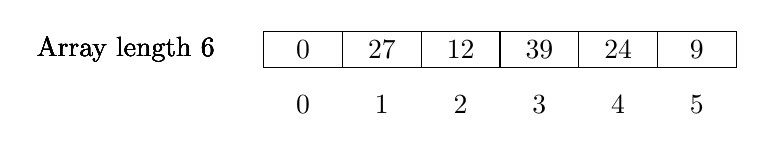
\begin{tikzpicture}
    \foreach \x [ evaluate={\l=int(mod(\x * 69, 42)}; ] in {0,...,5} {
      \node [left] at (-1,1) {Array length 6};
      \node [draw, minimum width=1cm] at (\x, 1) {$\l$};
      \node at (\x, 0.3) {\x};
    } % foreach
  \end{tikzpicture}
\end{center}

\begin{itemize}
  \item Access time: $\Theta (1)$
  \item Inserting $n$ items in the \textit{tail} for array size $n$: $\Theta(1)$ per item, $n \times \Theta(1) \in \Theta(1)$
  \item Inserting $n$ items in the \textit{tail} for array size \textit{unknown}: $\Theta(n)$ per item, $n \times \Theta(n) \in \Theta(n)$
  \item Resizing: $\Theta (n)$
\end{itemize}

Lesson? \textbf{Keep track of the size and the tail!}

\section{Linked List}

\begin{itemize}
  \item Access time: $\Theta (n)$
  \item Insertion: $\Theta(1)$
  \item Deletion:
    \begin{itemize}
      \item Singly LL: $O(n)$
      \item Singly Circular list: $O(n)$
      \item Doubly LL: $\Theta (1)$
      \item Doubly Circular list: $\Theta (1)$
    \end{itemize}
\end{itemize}

\section{Stack}

Stack takes the "last in, first out" approach.

\section{Queue}

Queue takes the "first in, first out" approach.

\section{Tree}

\begin{itemize}
  \item Search: $O(\log(n))$ for a balanced tree (right), $O(n)$ for unbalanced tree (left)
    \begin{multicols}{2}
      \begin{forest}
        for tree={ very thin, circle, draw },
        [{ $8$ } % lv 0
        %
        [{ $4$ }
        %
        [{ $2$ }
        [{ $1$ }]
        [{ $3$ }]
        ]
        %
        [{ $6$ }
        [{ $7$ }]
        ]
        ]
        %
        [{ $12$ }
        %
        [{ $10$ }
        [{ $9$ }]
        [{ $11$ }]
        ]
        %
        [{ $12$ }
        ]
        ]
        ]
      \end{forest}

      \begin{forest}
        for tree={ very thin, circle, draw },
        [{ $5$ } % lv 0
        [{ $4$ }
        [{ $3$ }
        [{ $2$ }
        [{ $1$ }
        ]
        ]
        ]
        ]
        [{}]
        ]
      \end{forest}
    \end{multicols}
  \item \textbf{Maximum number of leaves:} $2^{h}$, where $h$ is the height of the tree
  \item \textbf{Maximum number of nodes:} $\sum^{h}_{i=0} 2^i = 2^{h + 1} - 1$, where $h$ is the height of the tree
\end{itemize}

Following calculations and traversals will be explained using the following \textbf {full binary tree}.

\begin{center}
  \begin{forest}
    for tree={ very thin, circle, draw },
    [{ A } % lv 0
    %
    [{ B }
    %
    [{ D }]
    %
    [{ E }]
    ]
    %
    [{ C }
    %
    [{ F }]
    [{ G }]
    %
    ]
    ]
  \end{forest}
\end{center}

Definitions:

\begin{itemize}
  \item $I$ (number of internal nodes) $= 3$ (A, B, C -- root is an internal node unless it is a leaf)
  \item $N$ (number of nodes) $= 7$
  \item $L$ (number of leaves) $= 4$
\end{itemize}

Full binary tree properties:

\begin{itemize}
  \item $L = I + 1 = \frac{N + 1}{2}$
  \item $N = 2I + 1 = 2L - 1$
  \item $I = \frac{N - 1}{2} = L - 1$
\end{itemize}

Traversal (applicable for all trees, including non-full-binary trees):

\begin{itemize}
  \item \textbf{Preorder -- [N]ode [L]eft [R]ight:} A B D E C F G
  \item \textbf{Inorder -- [L][N][R]:} D B E A F C
  \item \textbf{Postorder -- [L][R][N]:} D E B F C A
  \item Level -- by height: A B C D E F
\end{itemize}

\section{Binary Heap}

\begin{itemize}
  \item Max heap: Key in each node is larger than or equal to the keys in node's two children
  \item Min heap: Key in each node is less than or equal to the keys in node's two children
\end{itemize}

Array implementation for the above max-heap is as follow:

\begin{itemize}
  \item \textproc{Left-child($i$)} = $2i + 1$
  \item \textproc{Right-child($i$)} = $2i + 2$
  \item \textproc{Parent($i$)} = $\lfloor \frac{i - 1}{2} \rfloor$, $i > 0$
\end{itemize}

\subsection{Building a Heap -- Top-down v.s. Bottom-up}
